\scanpage{31}

% The two long rules remain beside the page-reference column and text.
% Lower left termination is faint: the line is drawn only through the observed foot region.
\noindent
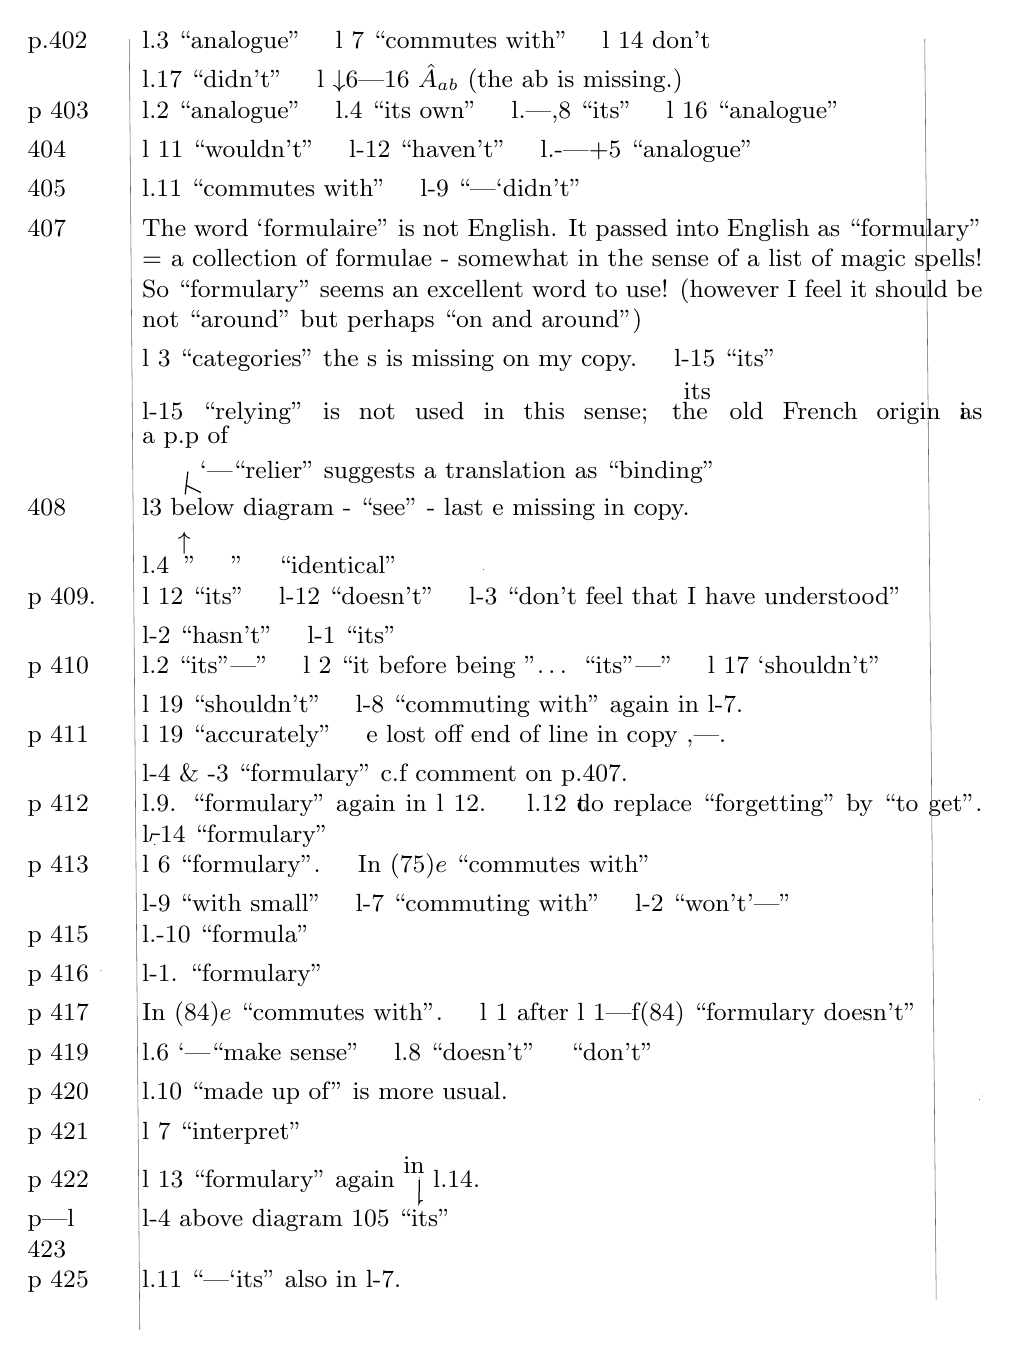
\begin{tikzpicture}
\node[anchor=north west,inner sep=0pt] (page031C) at (0,0) {%
\begin{minipage}{\linewidth}
\small
\begin{tabular}{@{}p{.095\linewidth}@{\hspace{.025\linewidth}}p{.88\linewidth}@{}}
p.402 & l.3 ``analogue'' \quad l 7 ``commutes with'' \quad l 14 don't\par\smallskip l.17 ``didn't'' \quad l \unsure{$\downarrow$6|16} $\hat{A}_{ab}$ (the ab is missing.) \\[.35em]
p 403 & l.2 ``analogue'' \quad l.4 ``its \deleted{own}'' \quad l\unsure{.|,}8 ``its'' \quad l 16 ``analogue'' \\[.35em]
404 & l 11 ``wouldn't'' \quad l-12 ``haven't'' \quad l.\unsure{-|+}5 ``analogue'' \\[.35em]
405 & l.11 ``commutes with'' \quad l-9 \unsure{``|`}didn't'' \\[.35em]
407 & The word `formulaire'' is not English. It passed into English as ``formulary'' $=$ a collection of formulae - somewhat in the sense of a list of magic spells! So ``formulary'' seems an excellent word to use! (however I feel it should be not ``around'' but perhaps ``on and around'')\par\smallskip l 3 ``categorie\uline{s}'' the s is missing on my copy. \quad l-15 ``its''\par\smallskip l-15 ``relying'' is not used in this sense; \tikz[baseline=(old407C.base)]{\node[inner sep=0pt] (old407C) {\deleted{the}};\node[anchor=south west,inner sep=0pt] at ([xshift=.45em,yshift=.15ex]old407C.north west) {\inserted{its}};} old French origin \tikz[baseline=(ias407C.base)]{\node[inner sep=0pt] (ias407C) {\deleted{i}};\node[anchor=base west,inner sep=0pt] at (ias407C.base west) {a};}s \tikz[baseline=(rel407C.base)]{\node[inner sep=0pt] (rel407C) {\unsure{`|``}relier''};\node[anchor=south,inner sep=0pt] at ([xshift=-.55em,yshift=1.1ex]rel407C.north west) {\inserted{a p.p of}};\draw[line width=.45pt,line cap=round] ([xshift=-.45em,yshift=.65ex]rel407C.base west)--([xshift=-.55em,yshift=-1.4ex]rel407C.base west);\draw[line width=.45pt,line cap=round] ([xshift=-.51em,yshift=-.6ex]rel407C.base west)--([xshift=.05em,yshift=-1.25ex]rel407C.base west);} suggests a translation as ``binding'' \\[.35em]
408 & l3 below diagram - ``see'' - last e missing in copy.\par\smallskip l.4 \tikz[baseline=(ditto408C.base)]{\node[inner sep=0pt] (ditto408C) {''};\node[anchor=south,inner sep=0pt] at ([xshift=-.25em,yshift=.15ex]ditto408C.north) {$\uparrow$};} \quad '' \quad \tikz[baseline=(id408C.base)]{\node[inner sep=0pt] (id408C) {``identical''};\fill ([xshift=3.3em,yshift=.4ex]id408C.base east) circle (.045ex);} \\[.35em]
p 409. & l 12 ``its'' \quad l-12 ``doesn't'' \quad l-3 ``don't feel that I have understood''\par\smallskip l-2 ``hasn't'' \quad l-1 ``its'' \\[.35em]
p 410 & \deleted{l.2} ``\deleted{its}\unsure{\deleted{''}|''} \quad l 2 ``it \uline{before} being ''\ldots{} ``\deleted{\unsure{its}}\unsure{\deleted{''}|''} \quad l 17 `shouldn't''\par\smallskip l 19 ``shouldn't'' \quad l-8 ``commuting with'' again in l-7. \\[.35em]
p 411 & l 19 ``accurately'' \quad e lost off end of line in copy \unsure{,|.}\par\smallskip l-4 \& -3 ``formulary'' c.f comment on p.407. \\[.35em]
p 412 & l.9. ``formulary'' again in l 12. \quad l.12 \tikz[baseline=(do412C.base)]{\node[inner sep=0pt] (do412C) {\deleted{\unsure{t}}};\node[anchor=base west,inner sep=0pt] at (do412C.base west) {d};}o replace ``forgetting'' by ``to get''. \quad l\tikz[baseline=0pt,x=1ex,y=1ex]{\draw[line width=.45pt,line cap=round] (.12,.15)..controls(.27,.4)and(.24,.65)..(.3,.78)--(1.0,.75);\fill (.57,-.2) circle (.065);}14 ``formulary'' \\[.35em]
p 413 & l 6 ``formulary''. \quad In $(75)e$ ``commutes with''\par\smallskip l-9 ``with small'' \quad l-7 ``commuting with'' \quad l-2 ``won't\unsure{'|''} \\[.35em]
p 415 & l.-10 ``formula'' \\[.35em]
\tikz[baseline=(p416C.base)]{\node[inner sep=0pt] (p416C) {p 416};\fill ([xshift=.45em,yshift=1.0ex]p416C.base east) circle (.04ex);} & l-1. ``formulary'' \\[.35em]
p 417 & In $(84)e$ ``commutes with''. \quad l 1 after \deleted{\unsure{l 1|f}}(84) ``formulary doesn't'' \\[.35em]
p 419 & l.6 \unsure{`|``}make sense'' \quad l.8 ``doesn't'' \quad ``don't'' \\[.35em]
p 420 & l.10 ``made up of'' is more usual.\hfill\tikz[baseline=0pt,x=1ex,y=1ex]{\fill (0,0) circle (.04);\fill (.22,.34) circle (.04);}\hspace{1.2em} \\[.35em]
p 421 & l 7 ``interpret'' \\[.35em]
p 422 & l 13 ``formulary'' again \tikz[baseline=0pt,x=1ex,y=1ex]{\path (0,0)--(.9,0);\node[anchor=south,inner sep=0pt] at (.1,1.2) {\inserted{in}};\draw[line width=.45pt,line cap=round] (.6,.68)--(.56,-1.5)..controls(.57,-1.35)and(.7,-1.22)..(.87,-1.23);\fill (.6,.88) circle (.045);} l.14. \\[.35em]
\unsure{p|l} 423 & l-4 above diagram 105 ``its'' \\[.35em]
p 425 & l.11 \unsure{``|`}its'' also in l-7. \\[.35em]
\end{tabular}
\end{minipage}};
\draw[black!60,line width=.2pt] ([xshift=.107\linewidth,yshift=-1.0ex]page031C.north west)--([xshift=.118\linewidth,yshift=-2.0ex]page031C.south west);
\draw[black!60,line width=.2pt] ([xshift=-.061\linewidth,yshift=-1.0ex]page031C.north east)--([xshift=-.049\linewidth,yshift=.5ex]page031C.south east);
\end{tikzpicture}
% archive sheet number: 30
